The web frontend is designed to provide an intuitive exploration of the different datasets, clustering algorithms and distances. In an interactive interface multiple clustering settings can be chosen and a visualisation of the results is directly generated. 
A cluster-table is used to store previous calculated results, which can be plotted within the evaluation module. \\
The checkbox \qq{Use precalculated results (with random seed for reproduction)} at the top of the page (see \autoref{fig:parameters} A), which is set by default, allows the use of precalculated clustering results, which have been computed beforehand (with a random seed value) and are stored in the github repository. This was done for reproduction and runtime purposes. The second checkbox "use interactive charts" (see \autoref{fig:parameters} B), also set by default, allows the option for interactive projection plots for \acrshort{pca}, \acrshort{t-SNE}, and the evaluation module.  \\
The user can choose between four datasets (see \autoref{fig:parameters} C), four distance measures (see \autoref{fig:parameters} E) and four different algorithms (see \autoref{fig:parameters} D) via a drop-down menu. If one of the K-Algorithms is chosen a value for the parameter k between 1 and 10 has to be set (see \autoref{fig:parameters} F). The default value for k is 3. If DBSCAN is chosen the user has to define a value for Eps and MinPts. (see \autoref{fig:dbscan_para} A). Additionally, a link to a webpage implementing the DBSCAN heuristic described in section \ref{dbscanheuristic} is shown. A short manual for this page is given in section \ref{heuristicmanual}. The parameter settings can be adjusted with interactive slider widgets. \\
\begin{figure}[H]
	\centering
	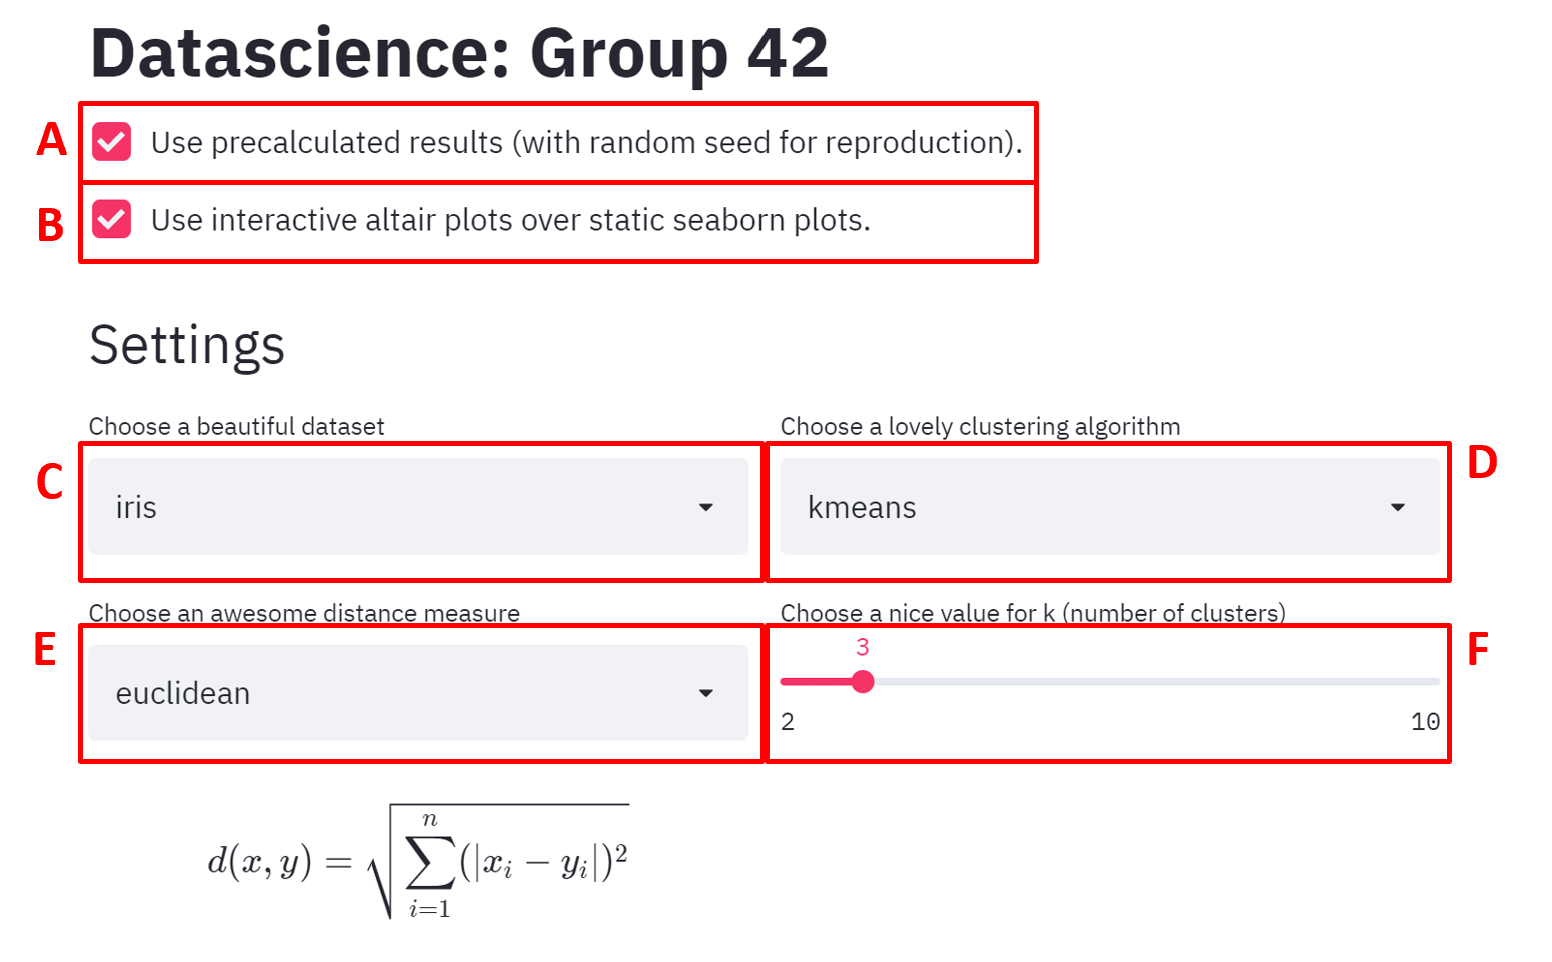
\includegraphics[width=\linewidth]{modules/web_frontend/eingabe_letters}
	\caption{First part of the web frontend. Setting options for clustering parameters for K-Means, K-Medians and K-Medoids.}\label{fig:parameters}
\end{figure}
\begin{figure}[H]
	\centering
	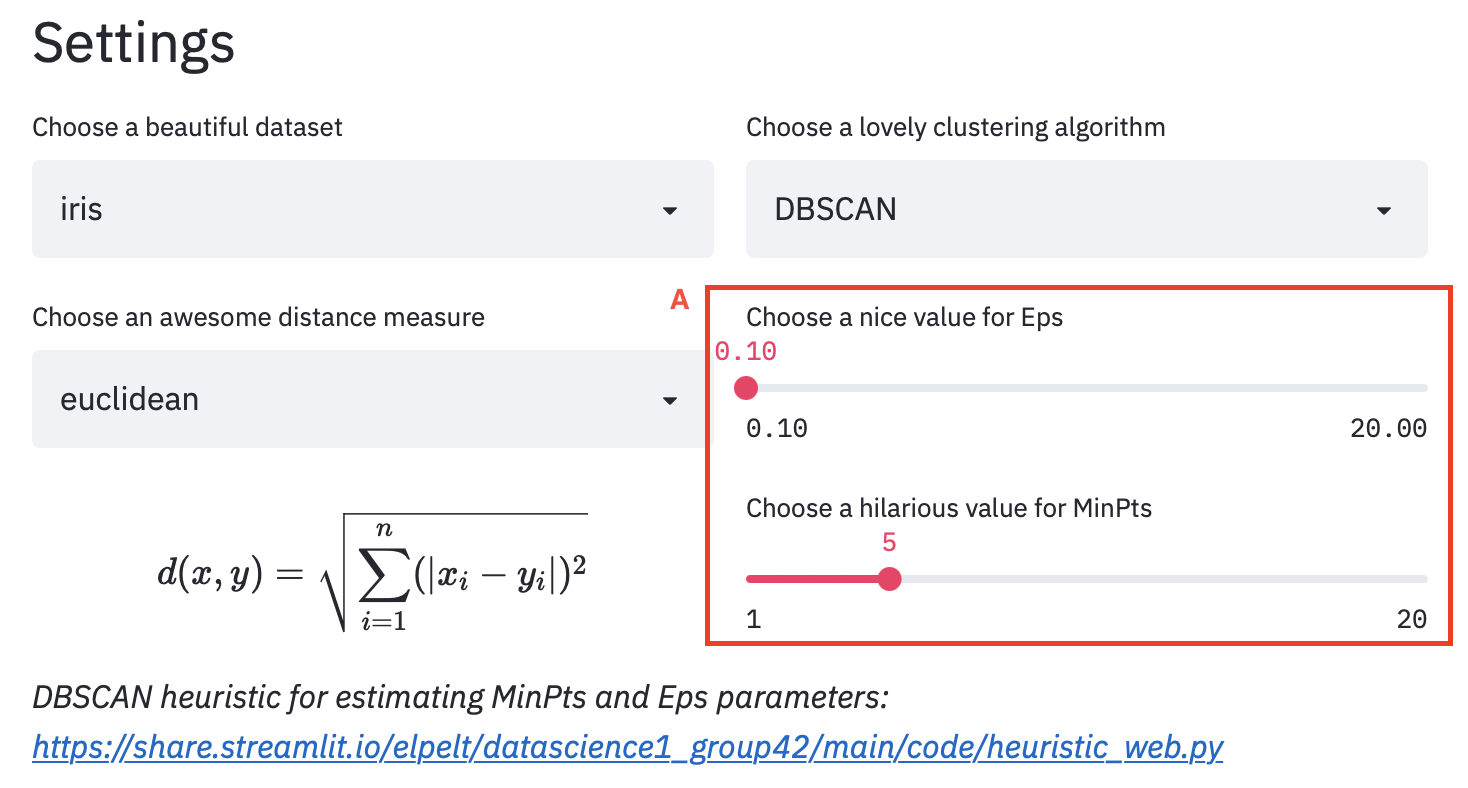
\includegraphics[width=\linewidth]{modules/web_frontend/DBSCAN_settings.png}
	\caption{Eps and MinPts setting options for DBSCAN.}\label{fig:dbscan_para}
\end{figure}

For every dataset detailed information can be retrieved via an expander widget. The dataset dimension (see \autoref{fig:data_info} A), pre classified cluster of the data (not for Diabetes dataset) (see \autoref{fig:data_info} B), datatypes per column (see \autoref{fig:data_info} C), dataset preview (see \autoref{fig:data_info} D), mean per column (see \autoref{fig:data_info} E), and optionally performed changes on the dataset are accessible.

\begin{figure}[H]
	\centering
	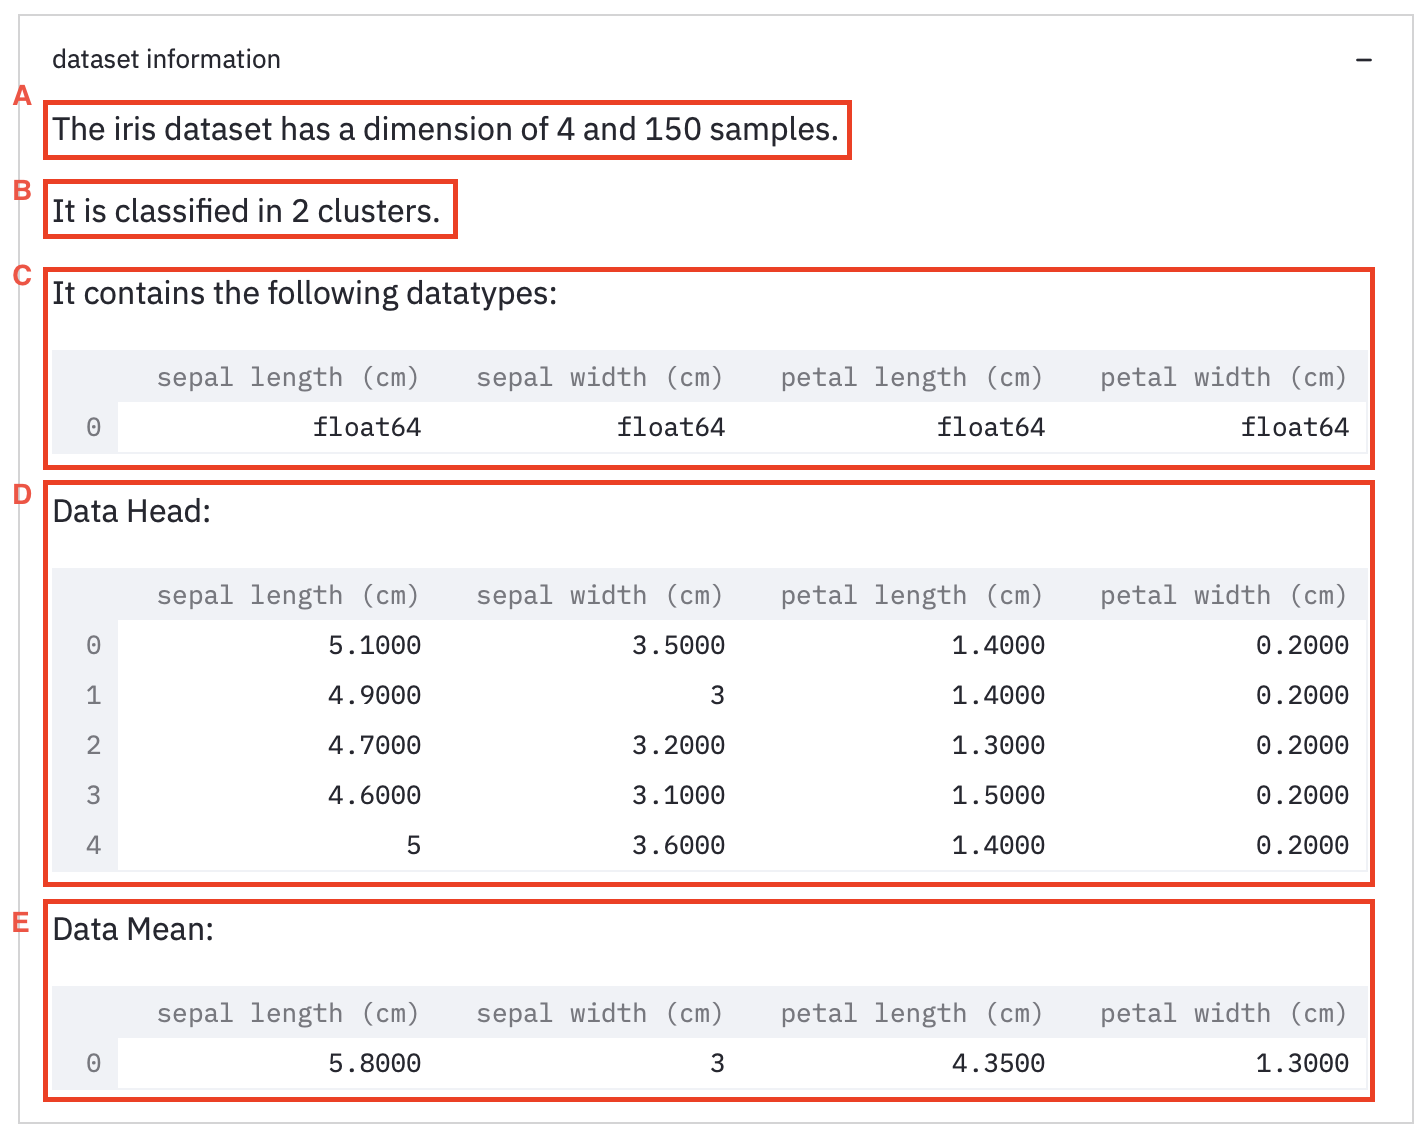
\includegraphics[width=\linewidth]{modules/web_frontend/dataset_inofs.png}
	\caption{Displayed dataset information by expanding the box. Iris dataset is shown as example.}\label{fig:data_info}
\end{figure}

Moreover the perplexity value for the \acrshort{t-SNE} projection can be set individually between 5 and 50 with a slider (see \autoref{fig:projection} A). The default value is 25. The \acrshort{t-SNE} and \acrshort{pca} plots are shown next to each other to allow a direct comparison of the lower-dimensional projections. For K-Medoids the medoid, for K-Means the mean, and for K-Medians the median for each cluster is marked as diamond (see \autoref{fig:projection} D). For the \acrshort{pca} plot both axes are labeled with the percentages of the first two component variances. To virtually interact with the plots, the button shown in \autoref{fig:projection} C can be clicked. Please note that this option is only available when the checkmark shown in \autoref{fig:parameters} B is set. Furthermore, this button provides the ability to save the plot in different formats.
When hovering over points in the plots a small window pops up displaying the cluster label and point index.
The calculated runtime is displayed right under the plots (see \autoref{fig:projection} B). This info is only accessible if precalculated results are not used (see \autoref{fig:parameters} A).
The frontend is reloaded entirely if a parameter value is changed, a different setting is made or a button is clicked. 
\begin{figure}[H]
	\centering
	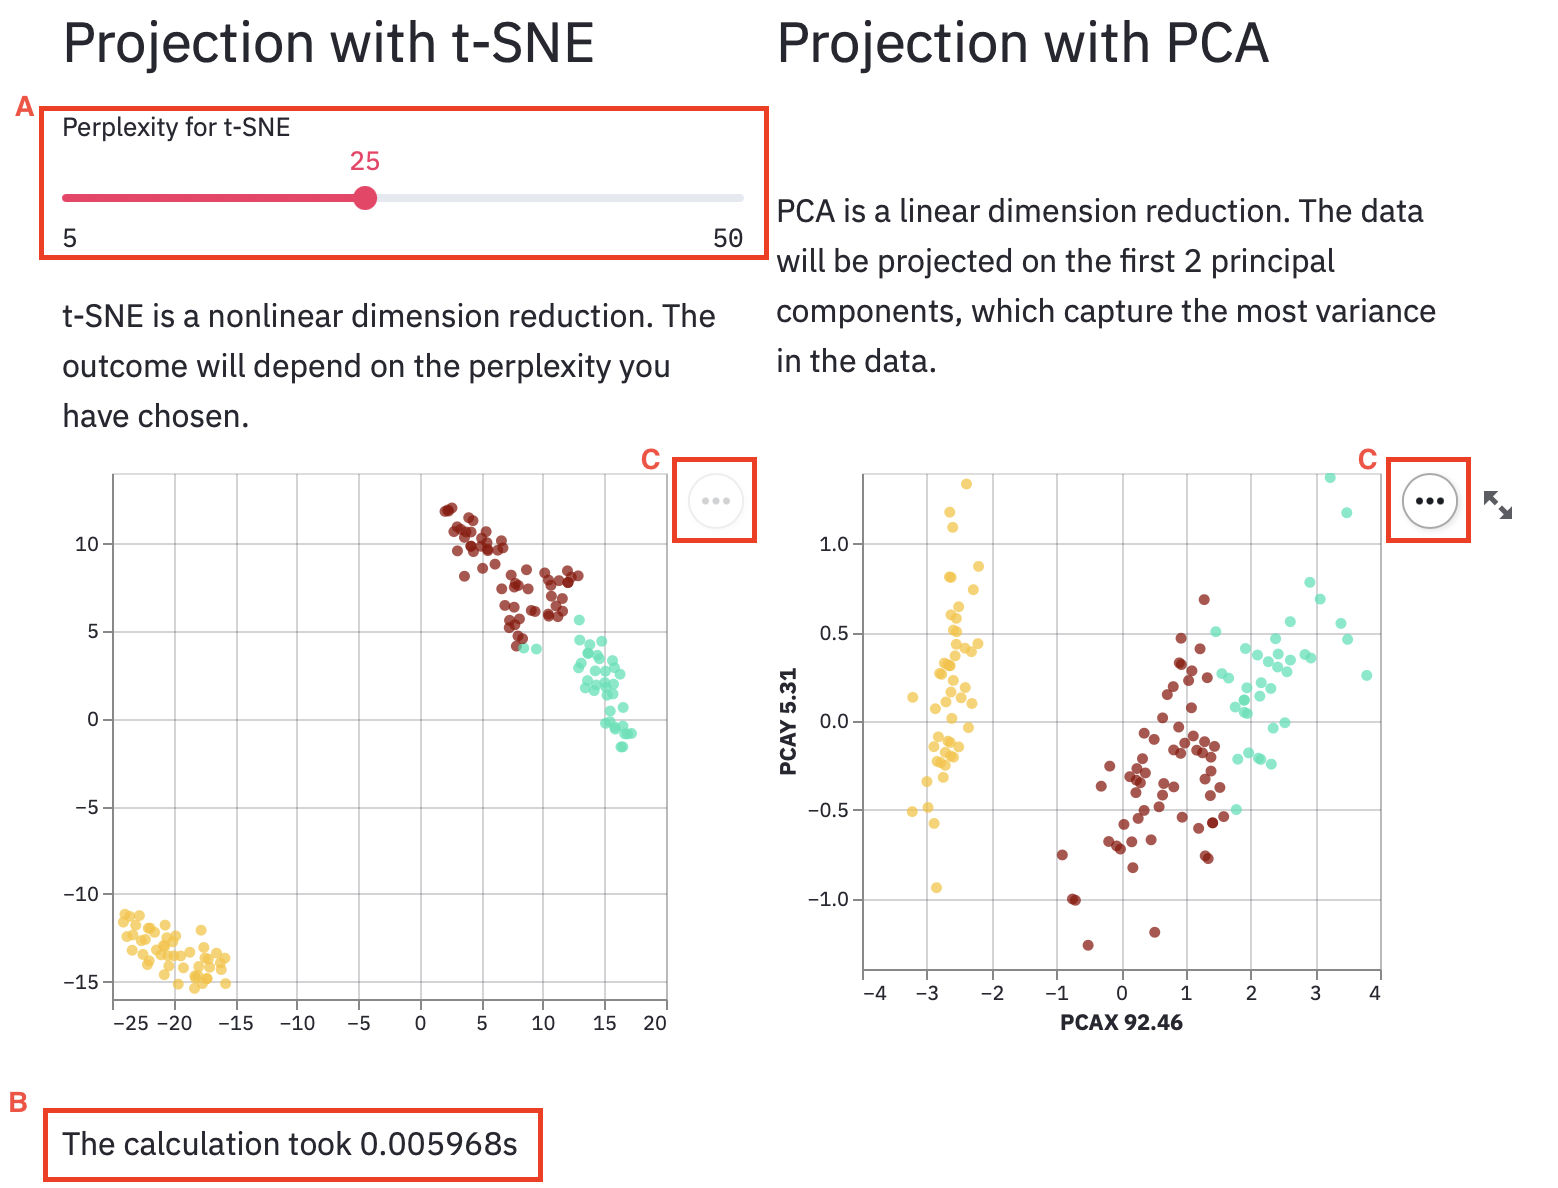
\includegraphics[width=\linewidth]{modules/web_frontend/projection_letters}
	\caption{Second part of the web frontend. Projection results of a clustering.}\label{fig:projection}
\end{figure}

The selected dataset can be viewed in a table format below the plots (see \autoref{fig:data_info_pca}).

\begin{figure}[H]
	\centering
	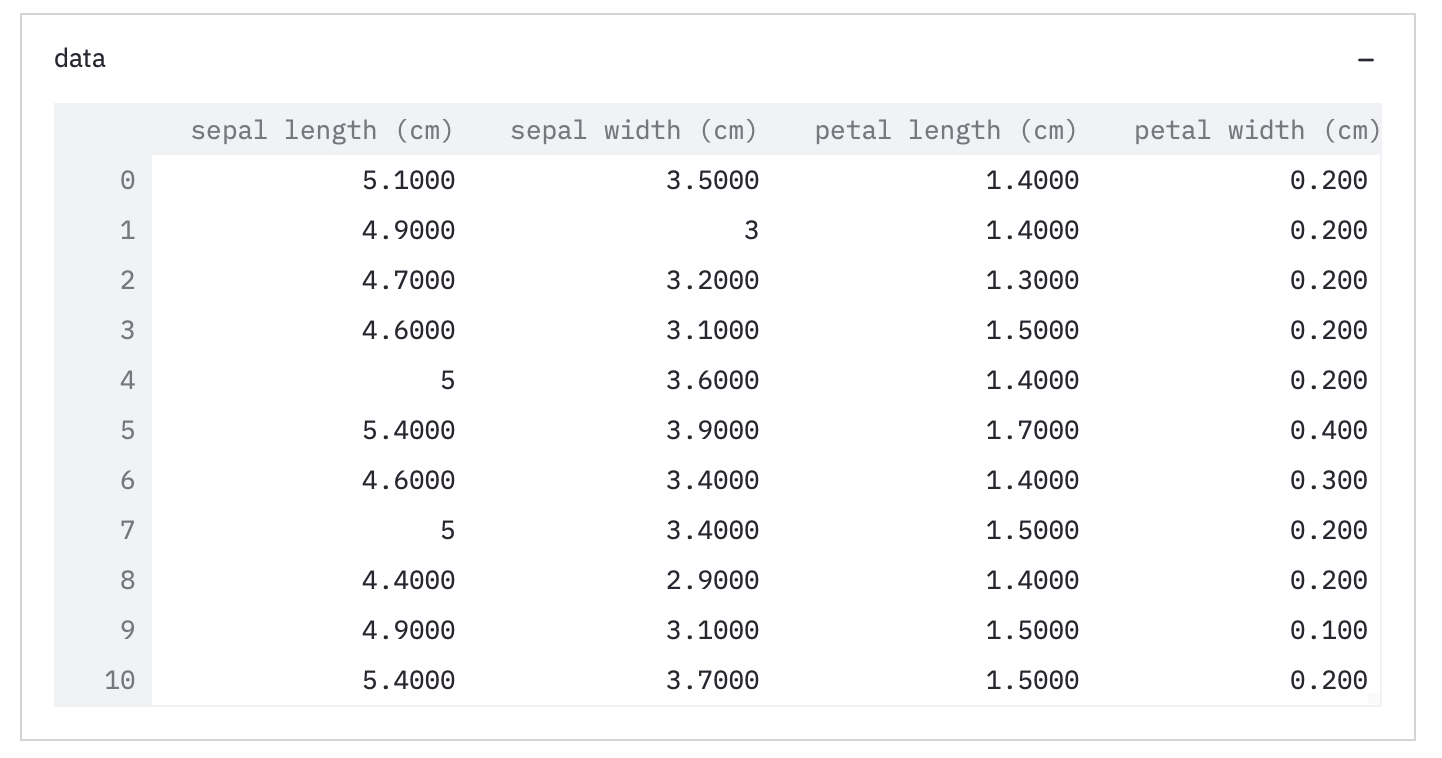
\includegraphics[width=\linewidth]{modules/web_frontend/data_info_pca.png}
	\caption{Projection of dataset as expander. Iris dataset as example.}\label{fig:data_info_pca}
\end{figure}

All clustering results can be saved in a cluster table for comparison via the \textit{Add}-button button (see \autoref{fig:evaluation} A). To compare this result to clusterings with other settings, the \textit{Add}-button can be clicked repeatedly after desired adjustment of the clustering settings. To start over and compare further clustering indices, the \textit{Reset}-button (see \autoref{fig:evaluation} B) can be clicked. The previous display of resulting indices will be cleared as well as the clustering table.
For the evaluation of the clustering results, one of five clustering indices can be chosen via a drop-down menu as shown in \autoref{fig:evaluation} C. An interactive barplot is displayed immediately, after adding a result to the cluster-table (see \autoref{fig:eval_bar}). The maximum reference value of 1 for the scores is also always displayed (see \autoref{fig:eval_bar} A). When hovering over the bars the score and the selected parameters for calculating the score are shown. When clicking on a bar only this bar is shown. Multiple bars can be selected by pressing shift and clicking.
\begin{figure}[H]
	\centering
	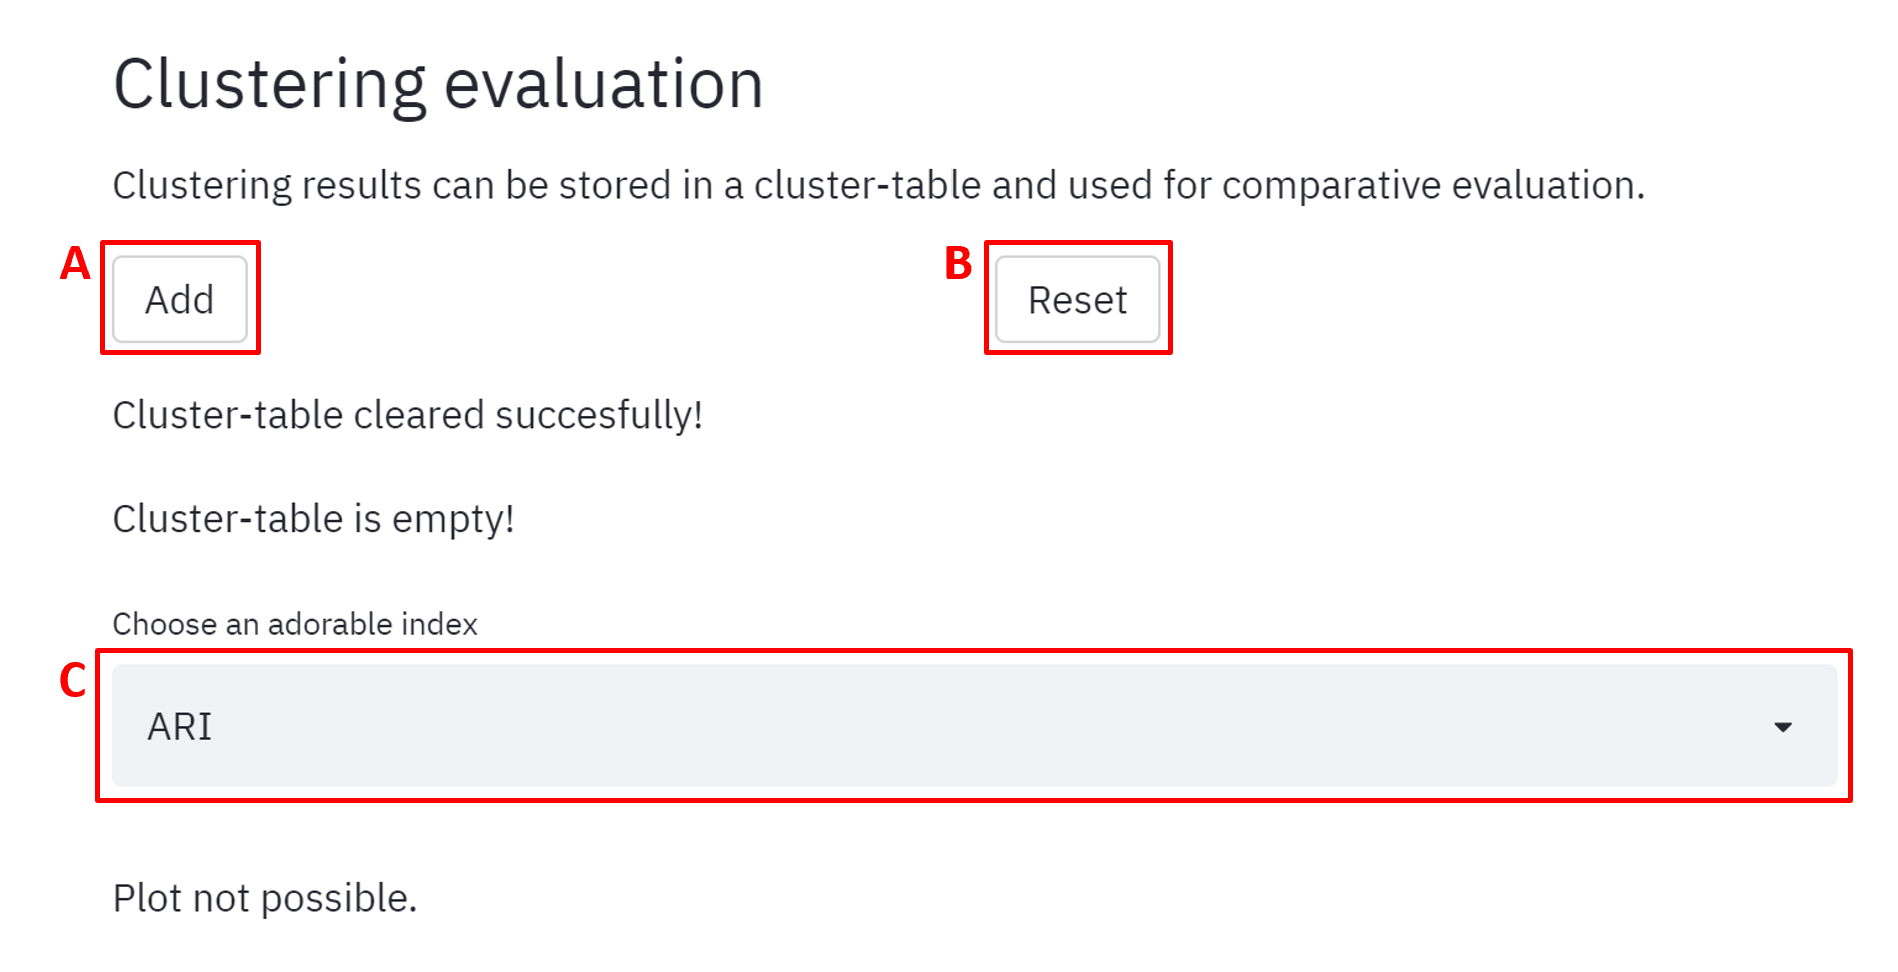
\includegraphics[width=\linewidth]{modules/web_frontend/evaluation_letters}
	\caption{Third part of the web frontend. Evaluation of clustering results.}\label{fig:evaluation}
\end{figure}

\begin{figure}[H]
	\centering
	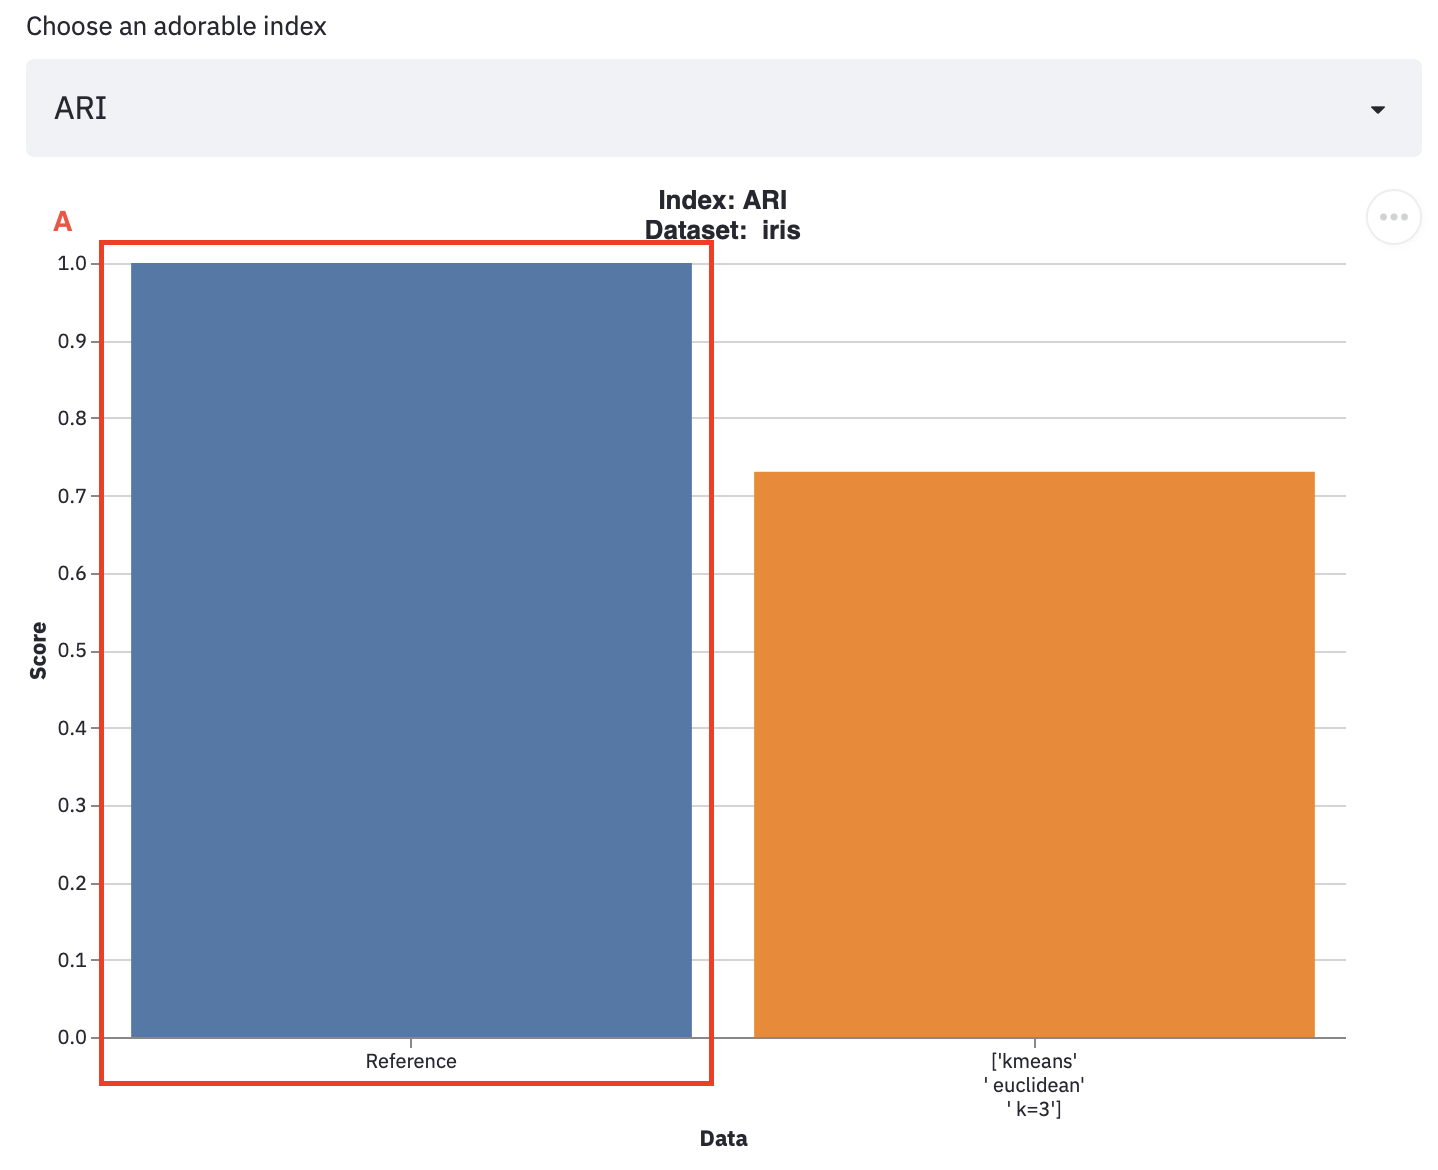
\includegraphics[width=0.75\textwidth]{modules/web_frontend/eval_bar.png}
	\caption{Barplot for evaluation comparison. K-Means, Euclidean, k=3, Iris, and \acrshort{ari} used as example.}\label{fig:eval_bar}
\end{figure}

Ancillary streamlit settings can be found at the upper right corner. Additional explanatory texts provide help and more information. \\


\subsection{DBSCAN Heuristic Page} \label{heuristicmanual}
The web frontend for calculating the sorted k-dist graph for the DBSCAN heuristic is build similarly to the main applications web frontend described above.
A simple form is presented where dataset, distance measure and the k value can be chosen using drop-down menus or sliders (see \autoref{fig:evaluation} A, B, C). (Note: k in this case is not the number of clusters. k stands for the k-nearest neighbour of any point)
Only when clicking the \textit{Calculate kdist Graph}-button (see \autoref{fig:evaluation} D) the sorted k-dist graph is calculated and plotted (see \autoref{fig:evaluation} E).

\begin{figure}[H]
	\centering
	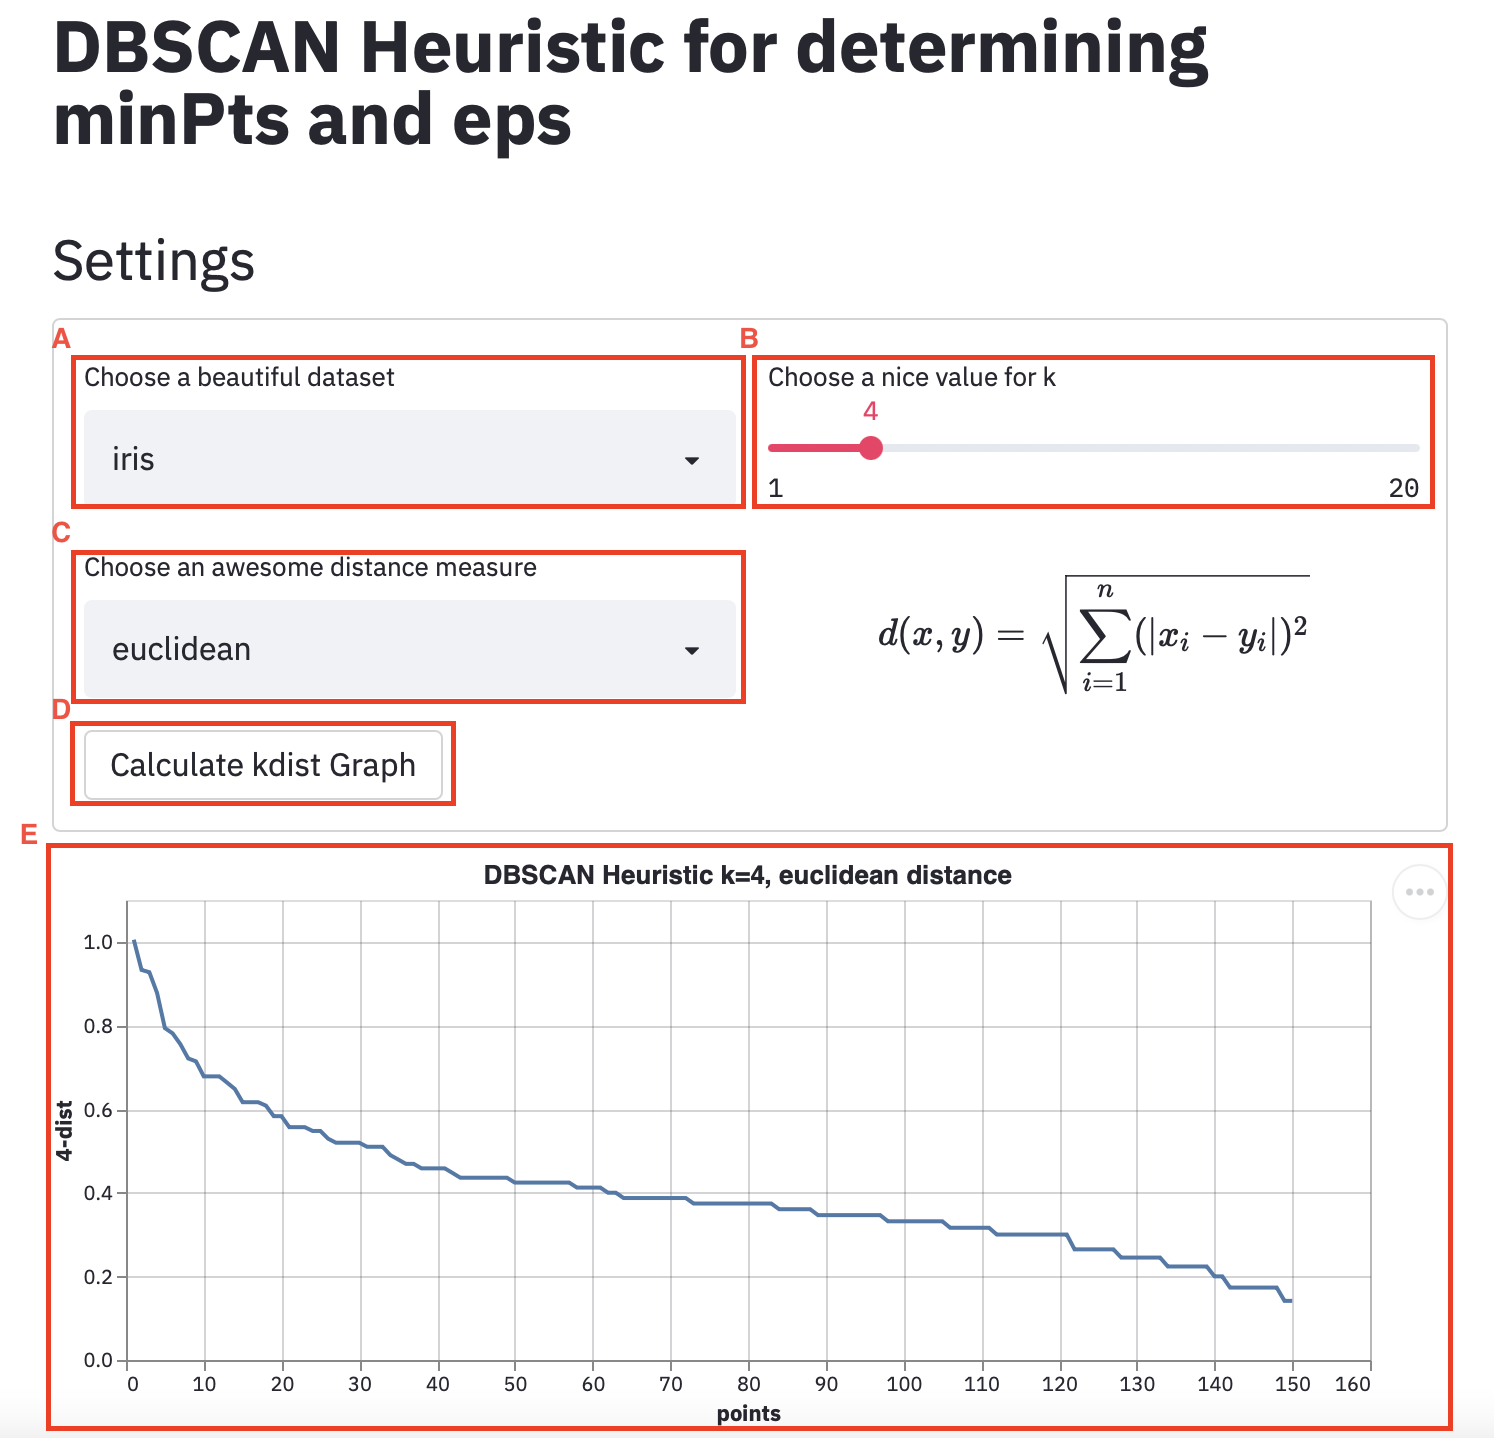
\includegraphics[width=\linewidth]{modules/web_frontend/dbscan_heuristic.png}
	\caption{DBSCAN heuristic settings}\label{fig:heuristicfrontend}
\end{figure}
